

\section{Combining Scores}

\begin{table}[b]
	\centering
\begin{tabular}{|llrr|}
\hline
Method & Family & SS score \quad  & \qquad PCA score \\ \hline

Simple corrected Viterbi	& Superfamily: & +72.7664 & \qquad +64.3552 \\ 
    						& Other:       & +21.8893 &  +17.2243 \\ \hline
Simple corrected forward	& Superfamily: & +71.0713 &  +50.0806 \\ 
    						& Other:       & +25.1106 &  +16.0857 \\ \hline


Reverse corrected Viterbi	& Superfamily: \qquad \qquad & +18.8087  &  +27.4886 \\ 
    						& Other:       & +0.56383 &  $-$0.41845 \\ \hline
Reverse corrected forward \qquad	& Superfamily: & +6.34041 & +21.3730 \\ 
    						& Other:       & +0.42186 & $-$0.55353 \\ \hline
\end{tabular}
	\caption{Average change for \acs{MSA} c.67.1 using primary structure only to the \acs{PCA} optimized score.}
	\label{tab:LST_ScoresPCA}
\end{table}




\acp{PCA} is a statistical approach that uses orthogonal transformation in order to reduce the dimensions of correlated data while preserving as much variability and thus information as possible (see \citep{Dunteman.1989}).
In consideration of the difference between the score with secondary structure information and those without, a linear combination of both scores might further improve the results. 
This is done by using \ac{PCA} to obtain the first principle component  of the two-dimensional data containing the score with and without secondary structure information. 


Table \ref{tab:LST_ScoresPCA} lists the average changes between the scores without secondary structure information and the first principal component of the same score, and the score including secondary structure. The column \textit{SS-Score} lists the average change without applying \ac{PCA} (see Table \ref{tab:LST_Scores}). Applying \ac{PCA} on both simple-corrected scores reduces the average change from the scores without secondary structure information by up to 36\,\%. In contrast, the superfamily scores for both reverse-corrected scores increase significantly, while the other scores decrease. 

The impact of using \ac{PCA} is shown in Figure \ref{fig:eval1CorrPCA} with scatterplots of the \ac{PCA}-generated scores over the scores with secondary structure. Both simple-corrected scores suffer from high deterioration. The scores in the transition region perform even more poorly, where the superfamily scores should separate from the other scores. On the other hand, the reverse-corrected scores provide a better result. The superfamily scores increase more than the other scores. Some of the reverse-corrected Viterbi scores decline in the transition area, but in the same region there is also a drop in the other scores.

\begin{figure}[H]
	\begin{center}
		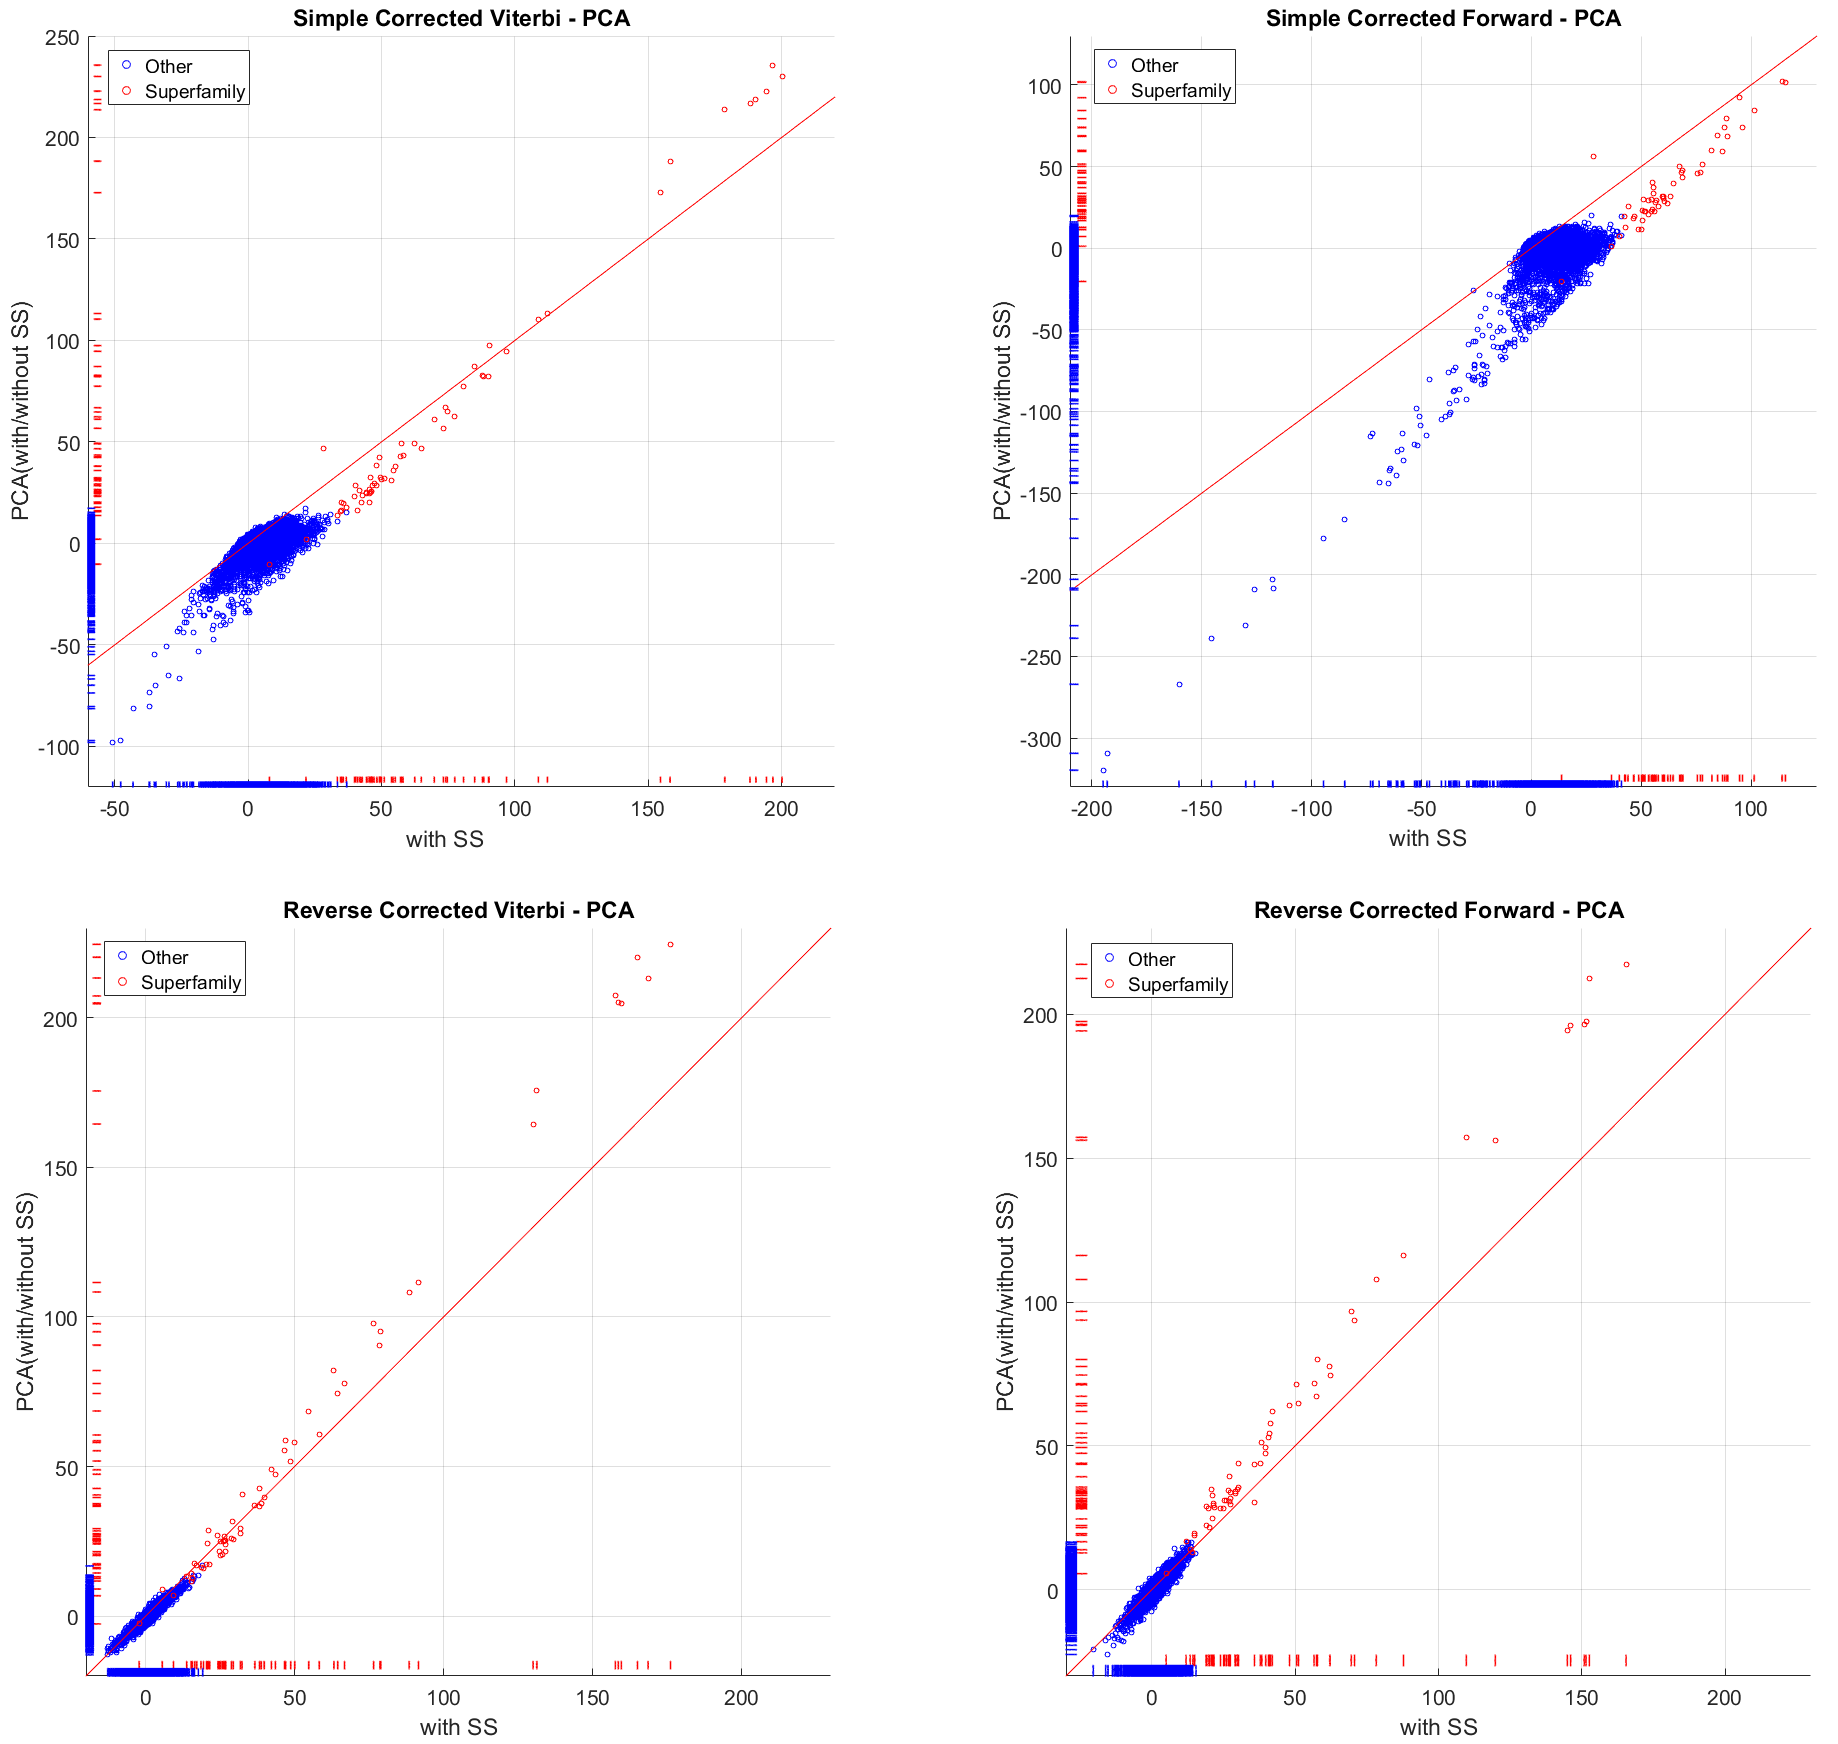
\includegraphics[width=0.9\textwidth]{fig/PCA/corr_pca}
	\end{center}
	\caption[Comparison of scores corrected by applying \acs{PCA}. ]{Comparison of scores corrected by applying \acs{PCA} over the secondary structure scores.}
	\label{fig:eval1CorrPCA}
\end{figure}


From the figures shown previously in this chapter, it is obvious that the scores for both methods, i.e. the Viterbi algorithm and the forward algorithm, are highly correlated. Therefore, a linear combination of the scores from the same type should reduce the dimensional complexity of the data by uniting the information from each method. 

\aclp{PCA} was applied separately on both simple-corrected and reverse-corrected scores. 
These new scores are shown in Figure \ref{fig:PCAcorrSame} on the vertical axis over their associated Viterbi score on the horizontal axis. The mostly linear distribution shows that scores from the same type but different methods mostly share the same information. An exception is the lower section of the scores not related to the \texttt{c.67.1} superfamily. The reason for this drop in scores can be found in the distribution of both scores, visualized in the rug plot in Figure \ref{fig:eval1_simp} on the vertical axis. While both superfamily scores are spread around the same region, the other scores from the forward algorithm are spread over four times the area compared to those from the Viterbi algorithm.  

\begin{figure}[H]
	\begin{center}
		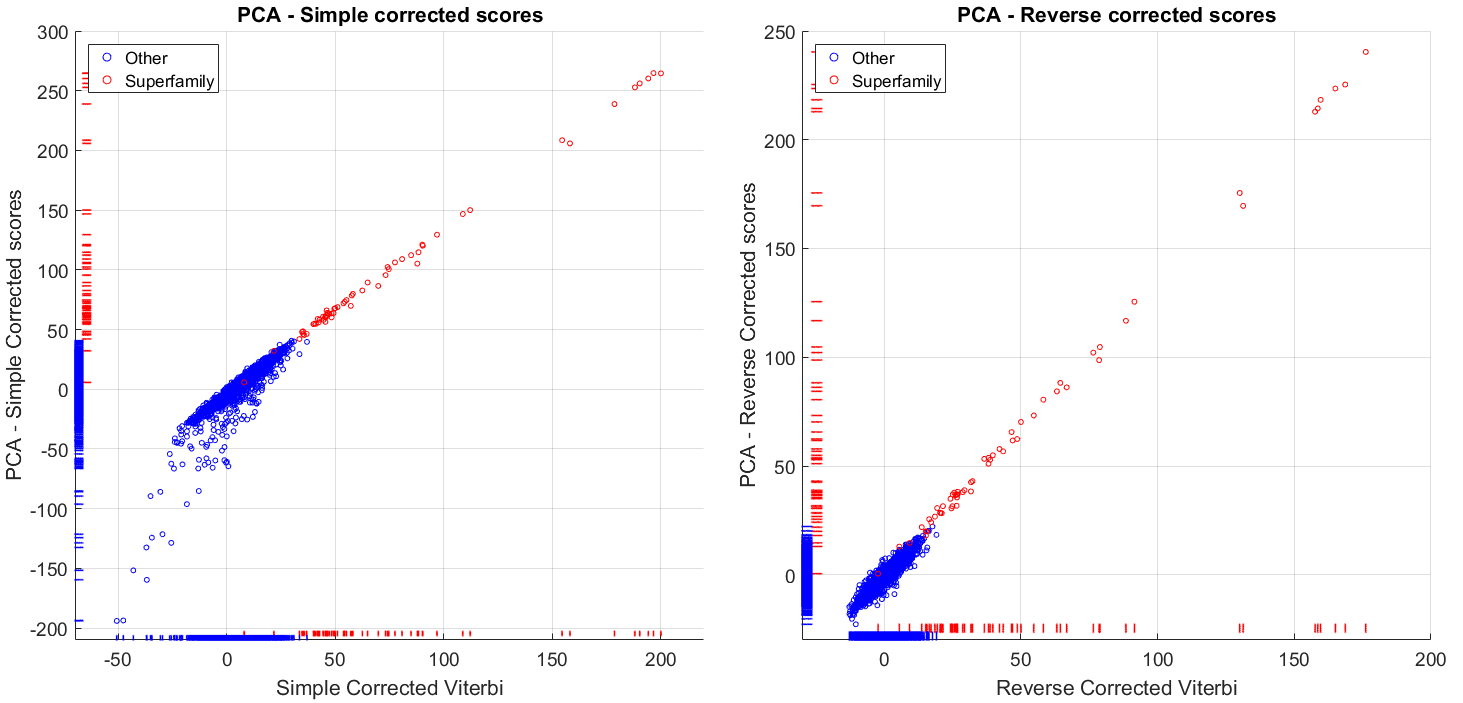
\includegraphics[width=\textwidth]{fig/PCA/pca_both_same}
	\end{center}
	\caption{\acs{PCA} applied to the scores over the Viterbi and forward methods.}
	\label{fig:PCAcorrSame}
\end{figure}

 

